% =======================================================
\chapter{Algorytmy ruchu indywidualnego w 3D}
% =======================================================

Przejście od nawigacji reaktywnej (sterowanie krok po kroku) do realizacji pełnych misji autonomicznych wymaga wykorzystania zaawansowanej algorytmiki i geometrii obliczeniowej. W tym rozdziale przedstawione zostaną trzy kanoniczne problemy robotyki mobilnej: planowanie pokrycia powierzchni (ang. \textit{Coverage Path Planning}), logistyczna optymalizacja trajektorii w grafach oraz przestrzenne przewidywanie ruchu obcych obiektów powietrznych.

\section{Geometria obliczeniowa w planowaniu misji (CPP)}

Problem Planowania Ścieżki Pokrycia (\textit{Coverage Path Planning} -- CPP) sprowadza się do znalezienia takiej trasy robota, która gwarantuje eksplorację zadanego obszaru $\mathcal{W}$ w całości, przy minimalizacji nadmiarowych przejść oraz zużycia energii. Zastosowanie CPP w lotnictwie bezzałogowym to przede wszystkim fotogrametria, rolnictwo precyzyjne (opryski) oraz operacje poszukiwawczo-ratownicze. Powszechnie stosowaną metodą rozwiązywania tego problemu jest klasyczny algorytm w kształcie meandra (wzór Boustrophedon / wzór Kosiarki).

\subsection{Algorytm zamiatania (Sweep-line) dla nieregularnych wielokątów}

Generowanie kosiarki dla idealnego, prostokątnego obszaru jest trywialne. Problem staje się obliczeniowo i analitycznie wymagający, gdy przestrzeń operacyjna $\mathcal{W}$ zadana jest jako dowolny wielokąt nieregularny, zdefiniowany przez uporządkowany zbiór wierzchołków $P = \{p_1, p_2, \dots, p_n\}$.

Aby ułożyć równoległe "paski" skanowania idealnie przycięte do obrysu pola (bez wylatywania drona poza wyznaczony teren, co marnowałoby cenną energię), stosuje się metodę \textbf{linii zamiatającej (ang. \textit{Sweep-line})}. 

\begin{figure}[ht]
    \centering
    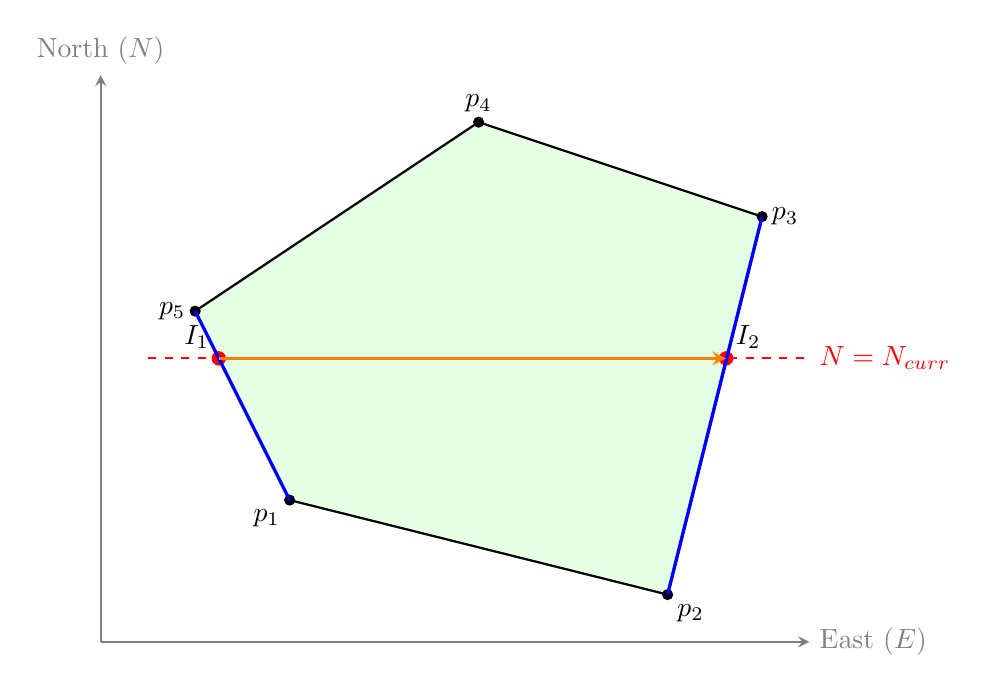
\begin{tikzpicture}[scale=1.2]
        % Wielokąt (Poligon)
        \draw[thick, fill=green!10] (0, 0) -- (4, -1) -- (5, 3) -- (2, 4) -- (-1, 2) -- cycle;
        
        % Węzły wielokąta
        \filldraw (0,0) circle (1.5pt) node[below left] {$p_1$};
        \filldraw (4,-1) circle (1.5pt) node[below right] {$p_2$};
        \filldraw (5,3) circle (1.5pt) node[right] {$p_3$};
        \filldraw (2,4) circle (1.5pt) node[above] {$p_4$};
        \filldraw (-1,2) circle (1.5pt) node[left] {$p_5$};
        
        % Oś Sweep-Line
        \draw[->, >=stealth, thick, gray] (-2, -1.5) -- (-2, 4.5) node[above] {North ($N$)};
        \draw[->, >=stealth, thick, gray] (-2, -1.5) -- (5.5, -1.5) node[right] {East ($E$)};
        
        % Pojedyncza linia Sweep
        \draw[dashed, red, thick] (-1.5, 1.5) -- (5.5, 1.5) node[right] {$N = N_{\text{curr}}$};
        
        % Punkty przecięcia
        \filldraw[red] (-0.75, 1.5) circle (2pt) node[above left, text=black] {$I_1$};
        \filldraw[red] (4.62, 1.5) circle (2pt) node[above right, text=black] {$I_2$};
        
        % Zaznaczenie przecinanych odcinków
        \draw[blue, very thick] (-1,2) -- (0,0);
        \draw[blue, very thick] (4,-1) -- (5,3);
        
        % Trasa kosiarki (Boustrophedon)
        \draw[->, >=stealth, orange, line width=1.2pt] (-0.75, 1.5) -- (4.62, 1.5);
    \end{tikzpicture}
    \caption{Zasada działania algorytmu Sweep-Line. Pozioma prosta (czerwona przerywana) przecina boki wielokąta, wyznaczając granice ścieżki przelotu (pomarańczowa strzałka) dla drona na danej osi rzędnych.}
    \label{fig:sweepline}
\end{figure}

\subsubsection{Matematyka punktu przecięcia}
Rozważmy poziomą prostą przesuwającą się wzdłuż osi North o z góry ustaloną wartość kroku $w$ (ang. \textit{swath width} -- wynikającą z szerokości obiektywu kamery). Z definicji, prosta pozioma ma równanie $N = N_{\text{curr}}$. 

Weźmy dowolny bok wielokąta łączący punkty $p_a = (N_a, E_a)$ oraz $p_b = (N_b, E_b)$. Warunkiem koniecznym przecięcia tego boku przez naszą prostą jest, aby rzędna $N_{\text{curr}}$ znajdowała się pomiędzy wierzchołkami odcinka:
\begin{equation}
    (N_a \le N_{\text{curr}} < N_b) \quad \lor \quad (N_b \le N_{\text{curr}} < N_a)
\end{equation}
Gdy ten warunek jest spełniony, rozwiązujemy równanie prostej przechodzącej przez dwa punkty dla zmiennej $E_{\text{intersect}}$:
\begin{equation}
    E_{\text{intersect}} = E_a + (E_b - E_a) \frac{N_{\text{curr}} - N_a}{N_b - N_a}
\end{equation}

Dla prostego, wypukłego wielokąta, algorytm znajdzie zawsze dokładnie dwa punkty przecięcia dla każdej linii (lewy i prawy skraj), tworząc w ten sposób precyzyjne odległości, po których dron wykona przelot. Zobacz implementację w skrypcie \texttt{07\_a\_polygon\_scan.py}.

\subsubsection{Algorytm wyznaczania trasy (Pseudokod)}
\begin{enumerate}
    \item Wyznacz wierzchołki ekstremalne wielokąta dla Bounding Boxa: $N_{\min}$ oraz $N_{\max}$.
    \item Zainicjalizuj $N_{\text{curr}} = N_{\min} + \frac{w}{2}$ oraz kierunek $D = 1$ (Lot w prawo).
    \item Dopóki $N_{\text{curr}} \le N_{\max}$:
    \begin{enumerate}
        \item Znajdź wszystkie boki, które przecina prosta $N_{\text{curr}}$ i wyznacz listę wartości $E$.
        \item Posortuj listę wartości $E$ rosnąco.
        \item Weź minimalną ($E_{\text{left}}$) i maksymalną ($E_{\text{right}}$) wartość.
        \item Jeśli $D = 1$, wygeneruj punkty trasy z lewej do prawej. W przeciwnym razie z prawej do lewej. (W celu optymalizacji nawrotów na bocznych krawędziach pola).
        \item Zmień kierunek: $D = D \times (-1)$. Zwiększ poziom linii: $N_{\text{curr}} += w$.
    \end{enumerate}
\end{enumerate}


\section{Optymalizacja grafowa: Problem Komiwojażera (TSP)}

W przypadku misji logistycznych (np. dostarczanie ładunków) trajektoria staje się grafem. Do optymalizacji takich problemów matematyka używa słynnego \textbf{Problemu Komiwojażera} (\textit{Traveling Salesperson Problem -- TSP}).

Niech $\mathcal{G} = (V, E)$ będzie grafem pełnym, gdzie zbiór wierzchołków $V$ określa losowo rozsiane punkty na ziemi, a zbiór krawędzi $E$ odpowiada bezpośrednim liniom przelotu drona między nimi. Koszt przelotu $c_{ij}$ przypisany krawędzi $(i,j)$ dany jest euklidesową odległością w przestrzeni. Oczekujemy znalezienia takiego cyklu Hamiltona (trasy, która odwiedzi każdy punkt dokładnie raz i wróci do bazy), aby zminimalizować sumę kosztów $\sum c_{ij}$.

Problem TSP jest obliczeniowo bardzo złożony (należy do klasy NP-trudnych). Dla $N$ wierzchołków istnieje $\frac{(N-1)!}{2}$ możliwych tras. O ile dla $N=8$ daje to zaledwie 2520 kombinacji, o tyle dla 20 paczek liczba ta przekracza moc obliczeniową standardowego komputera pokładowego drona.

\subsection{Przykład praktyczny: Heurystyka Najbliższego Sąsiada w logistyce}

Aby zapewnić działanie drona w czasie rzeczywistym i przy ograniczonych zasobach sprzętowych, rezygnujemy z poszukiwania globalnego absolutnego optimum i stosujemy algorytm przybliżony, używając koncepcji zachłannej (ang. \textit{Greedy Algorithm}).

W skrypcie \texttt{06\_tsp\_mission.py} zaimplementowano heurystykę Najbliższego Sąsiada (\textit{Nearest Neighbor}):
\subsubsection{Algorytm wyznaczania trasy (Pseudokod)}
\begin{enumerate}
    \item Wybierz punkt początkowy (Baza startowa drona).
    \item Dopóki na liście punktów nieodwiedzonych znajdują się lokalizacje:
    \begin{enumerate}
        \item Oblicz euklidesowe odległości od obecnej lokalizacji do wszystkich pozostałych.
        \item Wybierz punkt z \textbf{najmniejszą odległością}. (Akcja zachłanna).
        \item Udaj się do tego punktu, usuń go z listy i zapisz w tablicy trasy misji.
    \end{enumerate}
    \item Na koniec, dodaj odległość i drogę powrotu do Bazy.
\end{enumerate}
Algorytm ten generuje zadowalające trasy (często gorsze zaledwie o 15-20\% od doskonałego optimum), lecz wykonuje się w błyskawicznym czasie o złożoności $\mathcal{O}(N^2)$. Wyznaczona trasa zostaje wysłana komendą protokołu MAVLink bezpośrednio do pamięci EEPROM Autopilota, po czym uruchamia on bezstanowy lot w trybie \texttt{AUTO}.


\section{Matematyka naprowadzania predykcyjne (Lead Pursuit)}

Gdy wyznaczonym celem dla robota jest inny, poruszający się obiekt powietrzny (np. cel do sfilmowania z bliska lub nieautoryzowany dron do fizycznego przechwycenia), wgrane z góry misje na punktach (Waypointy) stają się bezużyteczne. Do sterowania w trybie \texttt{GUIDED} wykorzystuje się algorytmy naprowadzające, operujące bezpośrednio na wektorach prędkości przestrzennej $\mathbf{V}$.

Istnieją tu dwie filozofie podejścia:
\begin{itemize}
    \item \textbf{Pościg bezpośredni (Pure Pursuit):} Skrypt nieustannie rzutuje wektor kierunku z pozycji naszego drona na pozycję uciekającego celu (algorytm „pies goniący zająca”). Skutkuje to lotem tzw. \textit{krzywą pościgu}, na której dron zawsze ląduje "za ogonem" celu, dramatycznie wydłużając czas pościgu.
    \item \textbf{Naprowadzanie wyprzedzające (Lead Pursuit / Predictive Intercept):} Algorytm celuje w wirtualny punkt przestrzeni 3D, w którym cel dopiero się znajdzie. Dron ścina drogę, wykorzystując wektoryzację czasu.
\end{itemize}

\subsection{Rozwiązywanie problemu spotkania w 3D}

Oznaczmy nasz statek jako Dron (podskrypt $d$), a poruszający się cel jako Cel (podskrypt $c$).
Posiadamy informacje o pozycji $\mathbf{r}_d, \mathbf{r}_c$ oraz o prędkości uciekającego celu $\mathbf{v}_c$. Zakładamy, że nasz myśliwiec porusza się z maksymalną stałą prędkością skalarną $v_d = \|\mathbf{v}_d\|$. 

Naszym celem matematycznym jest znalezienie takiego kierunku lotu $\mathbf{\hat{v}}_d$, który doprowadzi do spotkania ($\mathbf{r}_d(t) = \mathbf{r}_c(t)$) w minimalnym czasie $t$.

\begin{figure}[ht]
    \centering
    \begin{tikzpicture}[scale=1.5]
        % Pozycje
        \coordinate (D) at (0,0);
        \coordinate (C) at (4,1);
        \coordinate (P) at (6,4);
        
        \filldraw[blue] (D) circle (1.5pt) node[below] {Dron $\mathbf{r}_d$};
        \filldraw[red] (C) circle (1.5pt) node[below right] {Cel $\mathbf{r}_c$};
        \filldraw[orange] (P) circle (1.5pt) node[above right] {Punkt Spotkania $\mathbf{P}(t)$};
        
        % Odległość początkowa i wektory lotu
        \draw[thick, gray, dashed] (D) -- (C) node[midway, below left] {$\mathbf{D} = \mathbf{r}_c - \mathbf{r}_d$};
        \draw[->, >=stealth, thick, red] (C) -- (P) node[midway, right] {$\mathbf{v}_c \cdot t$};
        \draw[->, >=stealth, thick, blue] (D) -- (P) node[midway, above left] {$\mathbf{v}_d \cdot t$};
        
    \end{tikzpicture}
    \caption{Trójkąt wektorowy wyprzedzającego punktu przechwycenia w 3D.}
    \label{fig:intercept}
\end{figure}

Zgodnie z Rysunkiem \ref{fig:intercept}, warunek spotkania w czasie $t$ możemy zapisać w postaci wektorowej (gdzie $\mathbf{D} = \mathbf{r}_c - \mathbf{r}_d$ to wektor dystansu początkowego):
\begin{equation}
    \mathbf{v}_d \cdot t = \mathbf{D} + \mathbf{v}_c \cdot t
\end{equation}
Obliczenie szukanego czasu do kolizji zmusza nas do podniesienia obu stron równania do kwadratu przy wykorzystaniu własności iloczynu skalarnego (pozbywamy się nieznanego kierunku $\mathbf{v}_d$, zostawiając znany nam, narzucony z góry skalar $v_d$):
\begin{align}
    (\mathbf{v}_d \cdot t)^2 &= (\mathbf{D} + \mathbf{v}_c t) \cdot (\mathbf{D} + \mathbf{v}_c t) \\
    v_d^2 t^2 &= \|\mathbf{D}\|^2 + 2 (\mathbf{D} \cdot \mathbf{v}_c) t + \|\mathbf{v}_c\|^2 t^2
\end{align}
Po przeniesieniu na jedną stronę otrzymujemy fundamentalne, sferyczne \textbf{równanie kwadratowe} naprowadzania:
\begin{equation}
    \underbrace{(v_d^2 - \|\mathbf{v}_c\|^2)}_{\text{Współczynnik } A} t^2 
    - \underbrace{2 (\mathbf{D} \cdot \mathbf{v}_c)}_{\text{Współczynnik } B} t 
    - \underbrace{\|\mathbf{D}\|^2}_{\text{Współczynnik } C} = 0
\end{equation}
Znajdując dodatni pierwiastek $t > 0$ tego równania (o ile wyróżnik $\Delta \ge 0$), potrafimy precyzyjnie wskazać punkt w przestrzeni trójwymiarowej $\mathbf{P}(t) = \mathbf{r}_c + \mathbf{v}_c \cdot t$, w którym cel znajdzie się dokładnie po tym czasie. Wystarczy teraz posłać naszego drona prosto w ten wyznaczony matematycznie wektor.

\subsection{Przykład praktyczny: Pościg i radary w skrypcie}
W środowisku testowym (skrypt \texttt{07\_b\_pursuit.py}) zastosowano wspomnianą algebrę dla uzyskania wysoce płynnego pościgu. Parametr czasu jest odczytywany asynchronicznie za pomocą polecenia `time.time()`, co minimalizuje ryzyko pomyłki fizyki wywołanej zacięciem okienka wyświetlającego na żywo renderowany model graficzny.

Dodatkowym elementem inżynieryjnym wdrożonym w tym ćwiczeniu jest technika spoofingu komunikacyjnego (tzw. złośliwe fałszowanie danych na radarze). Prawdziwy sprzęt lotniczy rozpoznaje pozycje intruzów za pomocą protokołu \textbf{ADS-B} (\textit{Automatic Dependent Surveillance–Broadcast}). MAVLink posiada wbudowaną komendę \texttt{adsb\_vehicle\_encode}. Przerzucając odczytane przez skrypt dane ruchomego obiektu UFO i wywołując tę komendę w stronę drona ścigającego, doprowadzamy do uaktywnienia się wirtualnych instrumentów GCS (\textit{Ground Control Station}). Dron (oraz Mapa MAVProxy) zostają skutecznie oszukane, że matematyczny zając jest prawdziwym, fizycznym samolotem znajdującym się w strefie przestrzeni powietrznej, co pozwala operatorowi wzrokowo koordynować akcję pościgową z poziomu okna konsoli.